\documentclass[slidetop,11pt]{beamer}
\hypersetup{pdfpagemode=FullScreen}

\usepackage{polyglossia}
\setdefaultlanguage{french}

\usepackage{xunicode,xltxtra}
%\usepackage{fontspec}
%\defaultfontfeatures{Mapping=tex-text,Scale=MatchLowercase}
\setmainfont{DejaVu Sans}
%\usepackage{graphicx}
\usepackage{url,hyperref}
%\usepackage{minted}

\useinnertheme[shadow=true]{rounded}
\useoutertheme{infolines}
\usecolortheme{dolphin}
\setbeamerfont{block title}{size={}}

\title{Soutenance de stage}
\subtitle{Sierra Wireless, Solutions \& Services \\ ~ \\ Maître de stage: Benjamin Cabé}
\author{Guilhem Saurel}
\institute{INP-ENSEEIHT}
\date{\today}
\logo{
\includegraphics[height=0.5cm]{../../images/inp-enseeiht}}


\begin{document}

\frame{\titlepage}

\begin{frame}{Sommaire}
    \small \tableofcontents
\end{frame}

\section{L’entreprise}

\begin{frame}
    \frametitle{Sommaire}
    \tableofcontents[currentsection, hideothersubsections]
\end{frame}

\subsection{Historique}
\begin{frame}
    \frametitle{Historique}
    \begin{itemize}
        \item Anyware Technologies
            
\includegraphics[width=3cm]{img/anyware-tech.png}
        \item Wavecom
            
\includegraphics[width=3cm]{img/wavecom.jpg}
        \item Sierra Wireless
            
\includegraphics[width=3cm]{img/swir.jpg}
    \end{itemize}
\end{frame}

\subsection{Présentation globale}
\begin{frame}
    \frametitle{Sierra Wirless}
    \begin{itemize}
        \item Originaire de Richmond (Canada)
        \item Leader en solutions embarquées sans fil (2G, 3G \& 4G), et plus récement en M2M/IoT
        \item Cotée en bourse (NASDAQ: SWIR, TSX: SW)
    \end{itemize}
\end{frame}

\subsection{Présentation locale}
\begin{frame}
    \frametitle{Sierra Wirless, Solutions \& Services}
    \begin{itemize}
        \item Développement logiciel, firmware \& web
        \item Support
        \item Administration système
    \end{itemize}
\end{frame}

\section{Mihini}

\begin{frame}
    \frametitle{Sommaire}
    \tableofcontents[currentsection, hideothersubsections]
\end{frame}

\subsection{Présentation}
\begin{frame}
    \frametitle{Contexte \& Présentation}
    \begin{block}{M2M.eclipse.org}
        
\includegraphics[width=3cm]{img/M2M.png}
    \end{block}
    \begin{block}{Mihini}
        
\includegraphics[width=3cm]{img/mihini_logo.png}
    \end{block}
\end{frame}

\subsection{Réalisation} %  TODO
\begin{frame}
    \frametitle{CMake / CPack}
    \begin{block}{Plateformes}
        \begin{itemize}
            \item Raspberry Pi
            \item Beagle Bone
            \item amd64 \& i386
        \end{itemize}
    \end{block}
    \begin{block}{Systèmes d’exploitation}
        \begin{itemize}
            \item Debian (et dérivées)
            \item Angstrom
            \item ArchLinux
            \item Fedora
            \item autres
        \end{itemize}
    \end{block}
\end{frame}


\subsection{Conclusion} %  TODO
\begin{frame}
    \frametitle{Résultats \& Intégration}
    \begin{itemize}
        \item Travail effectué sur Github (http://github.com/nim65s/mihini-repo)
            
\includegraphics[width=3cm]{img/github.png}
        \item ~20 commits
        \item plus de 1500 lignes ajoutées ou supprimées
        \item Intégré au repository officiel eclipse (http://git.eclipse.org/c/mihini/org.eclipse.mihini.git/log/?h=cpack)
    \end{itemize}
\end{frame}

\section{Eclo}

\begin{frame}
    \frametitle{Sommaire}
    \tableofcontents[currentsection, hideothersubsections]
\end{frame}

\subsection{Présentation}
\begin{frame}
    \frametitle{A "Connected Greenhouse"}
    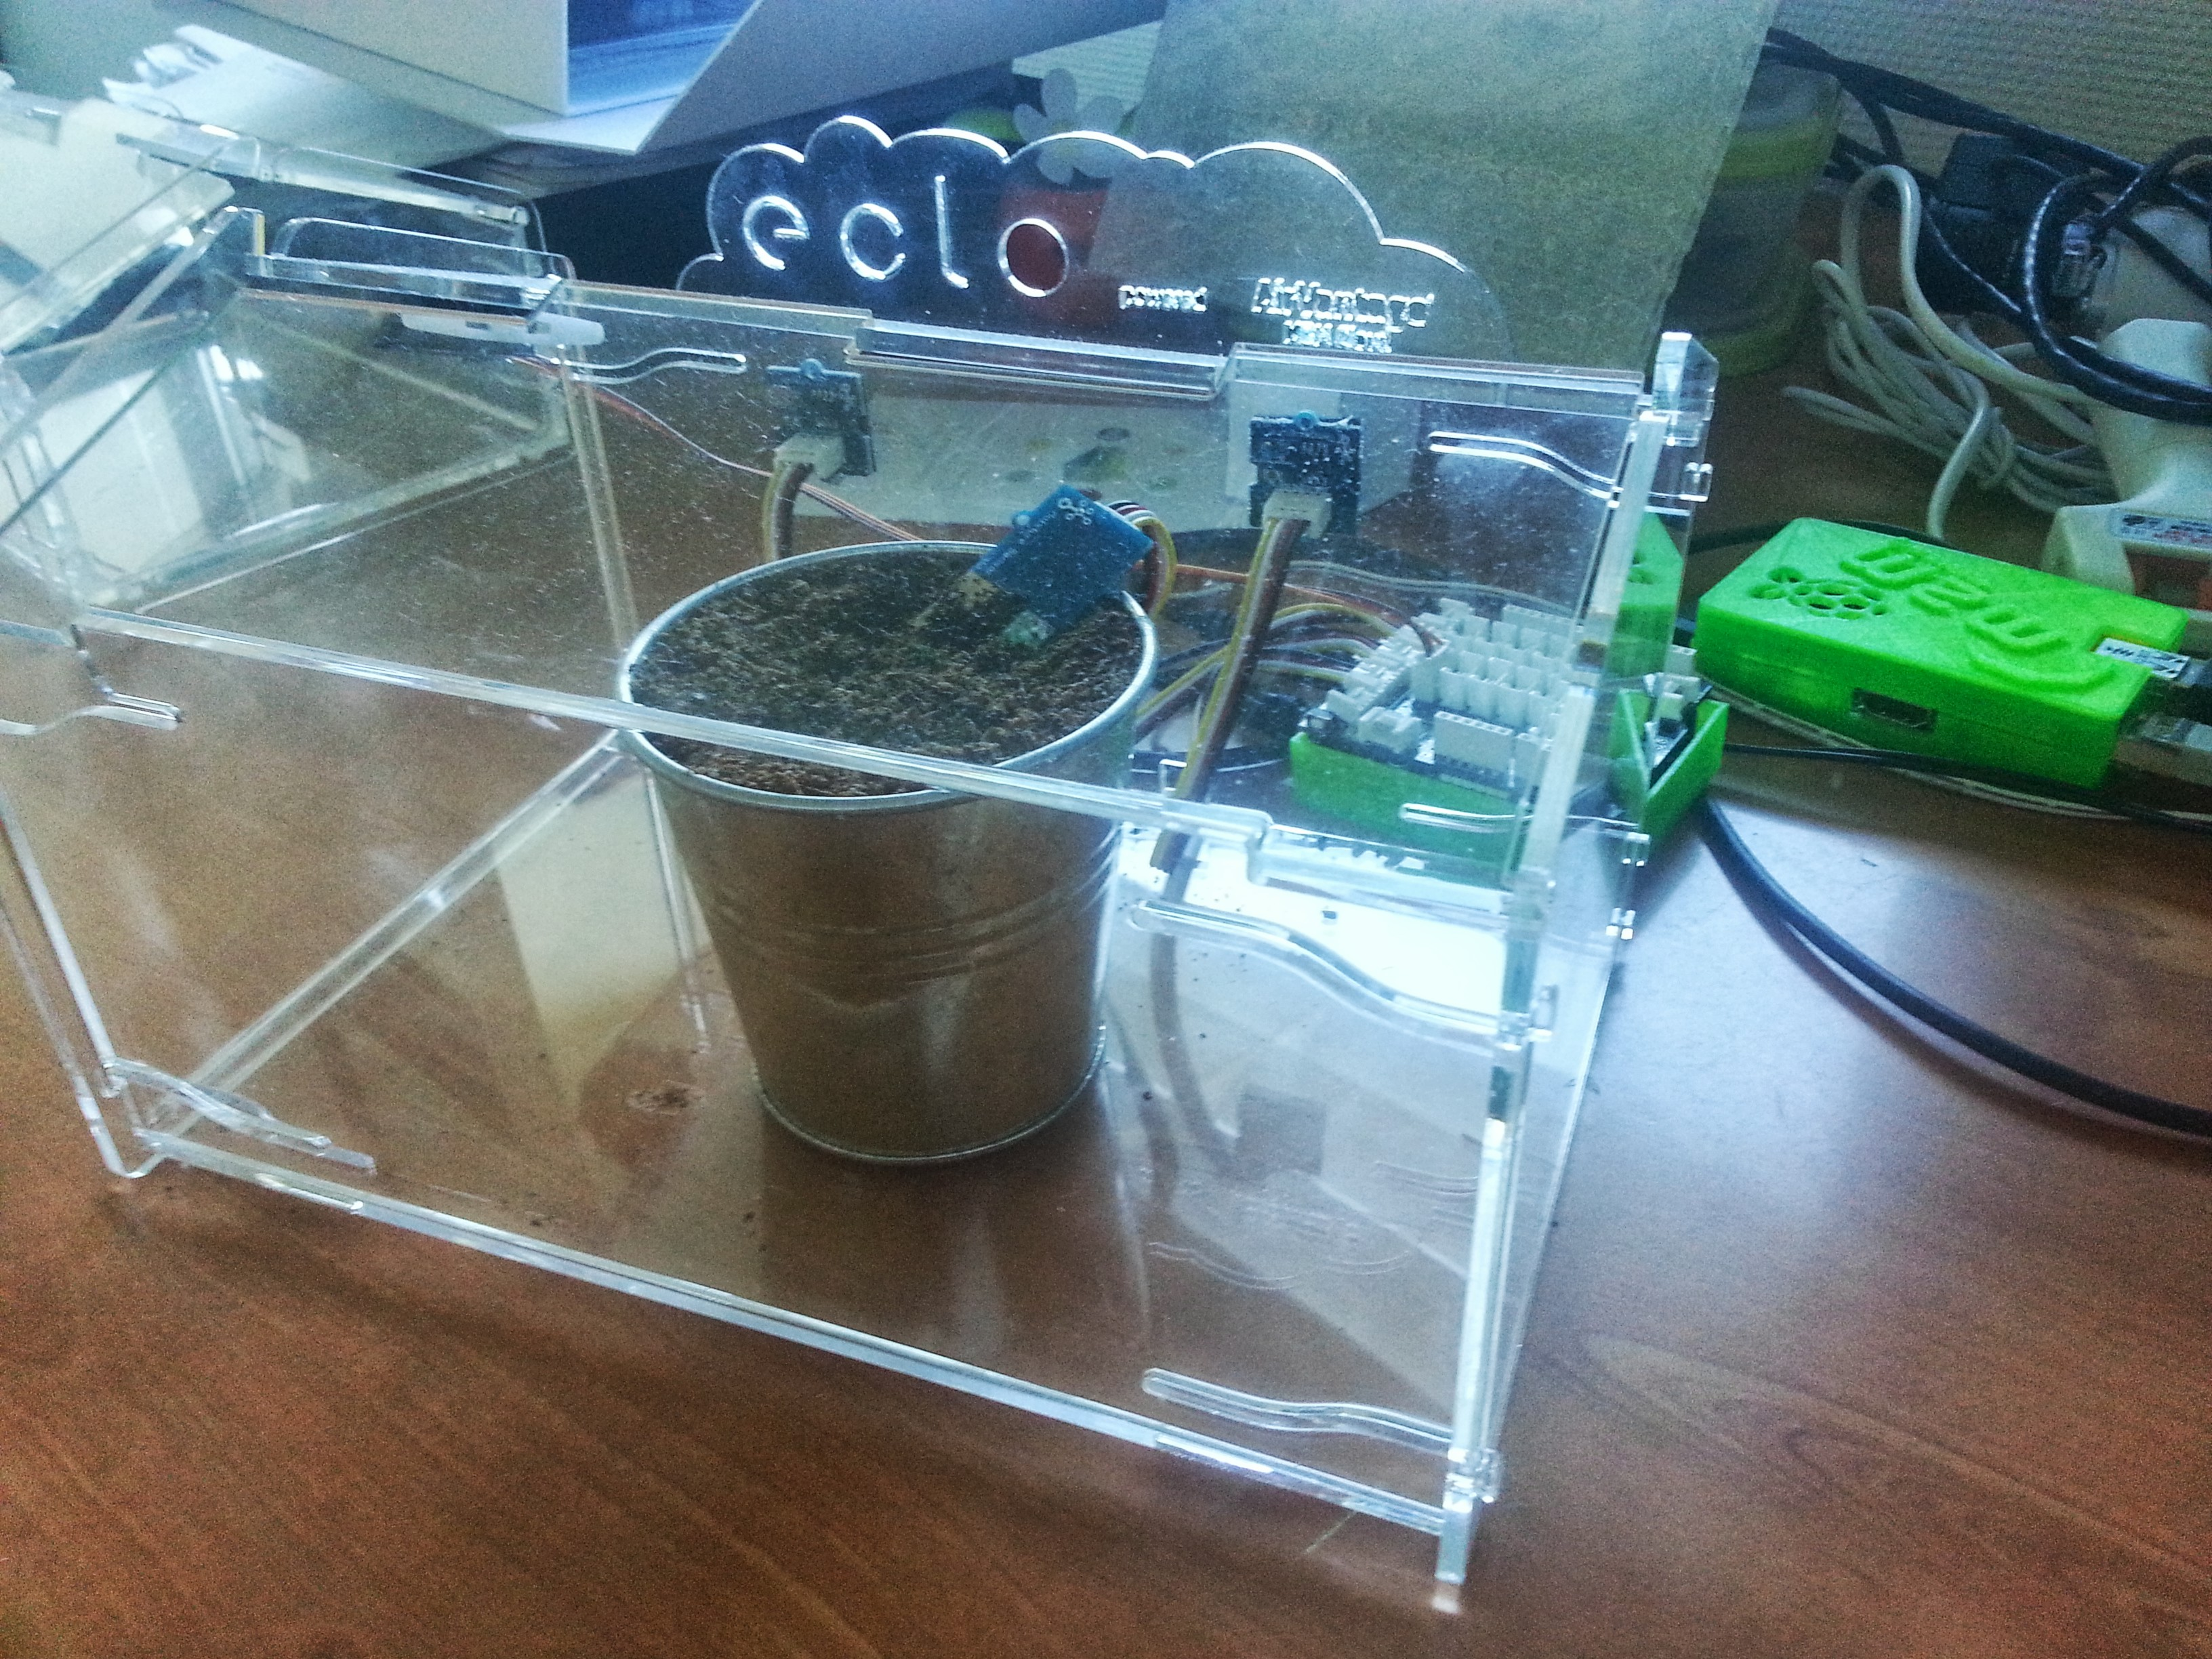
\includegraphics[width=\linewidth]{img/eclo.jpg}
\end{frame}

\subsection{Tutoriel}
\begin{frame}
    \frametitle{"End to end"}
    \begin{itemize}
        \item Arduino
            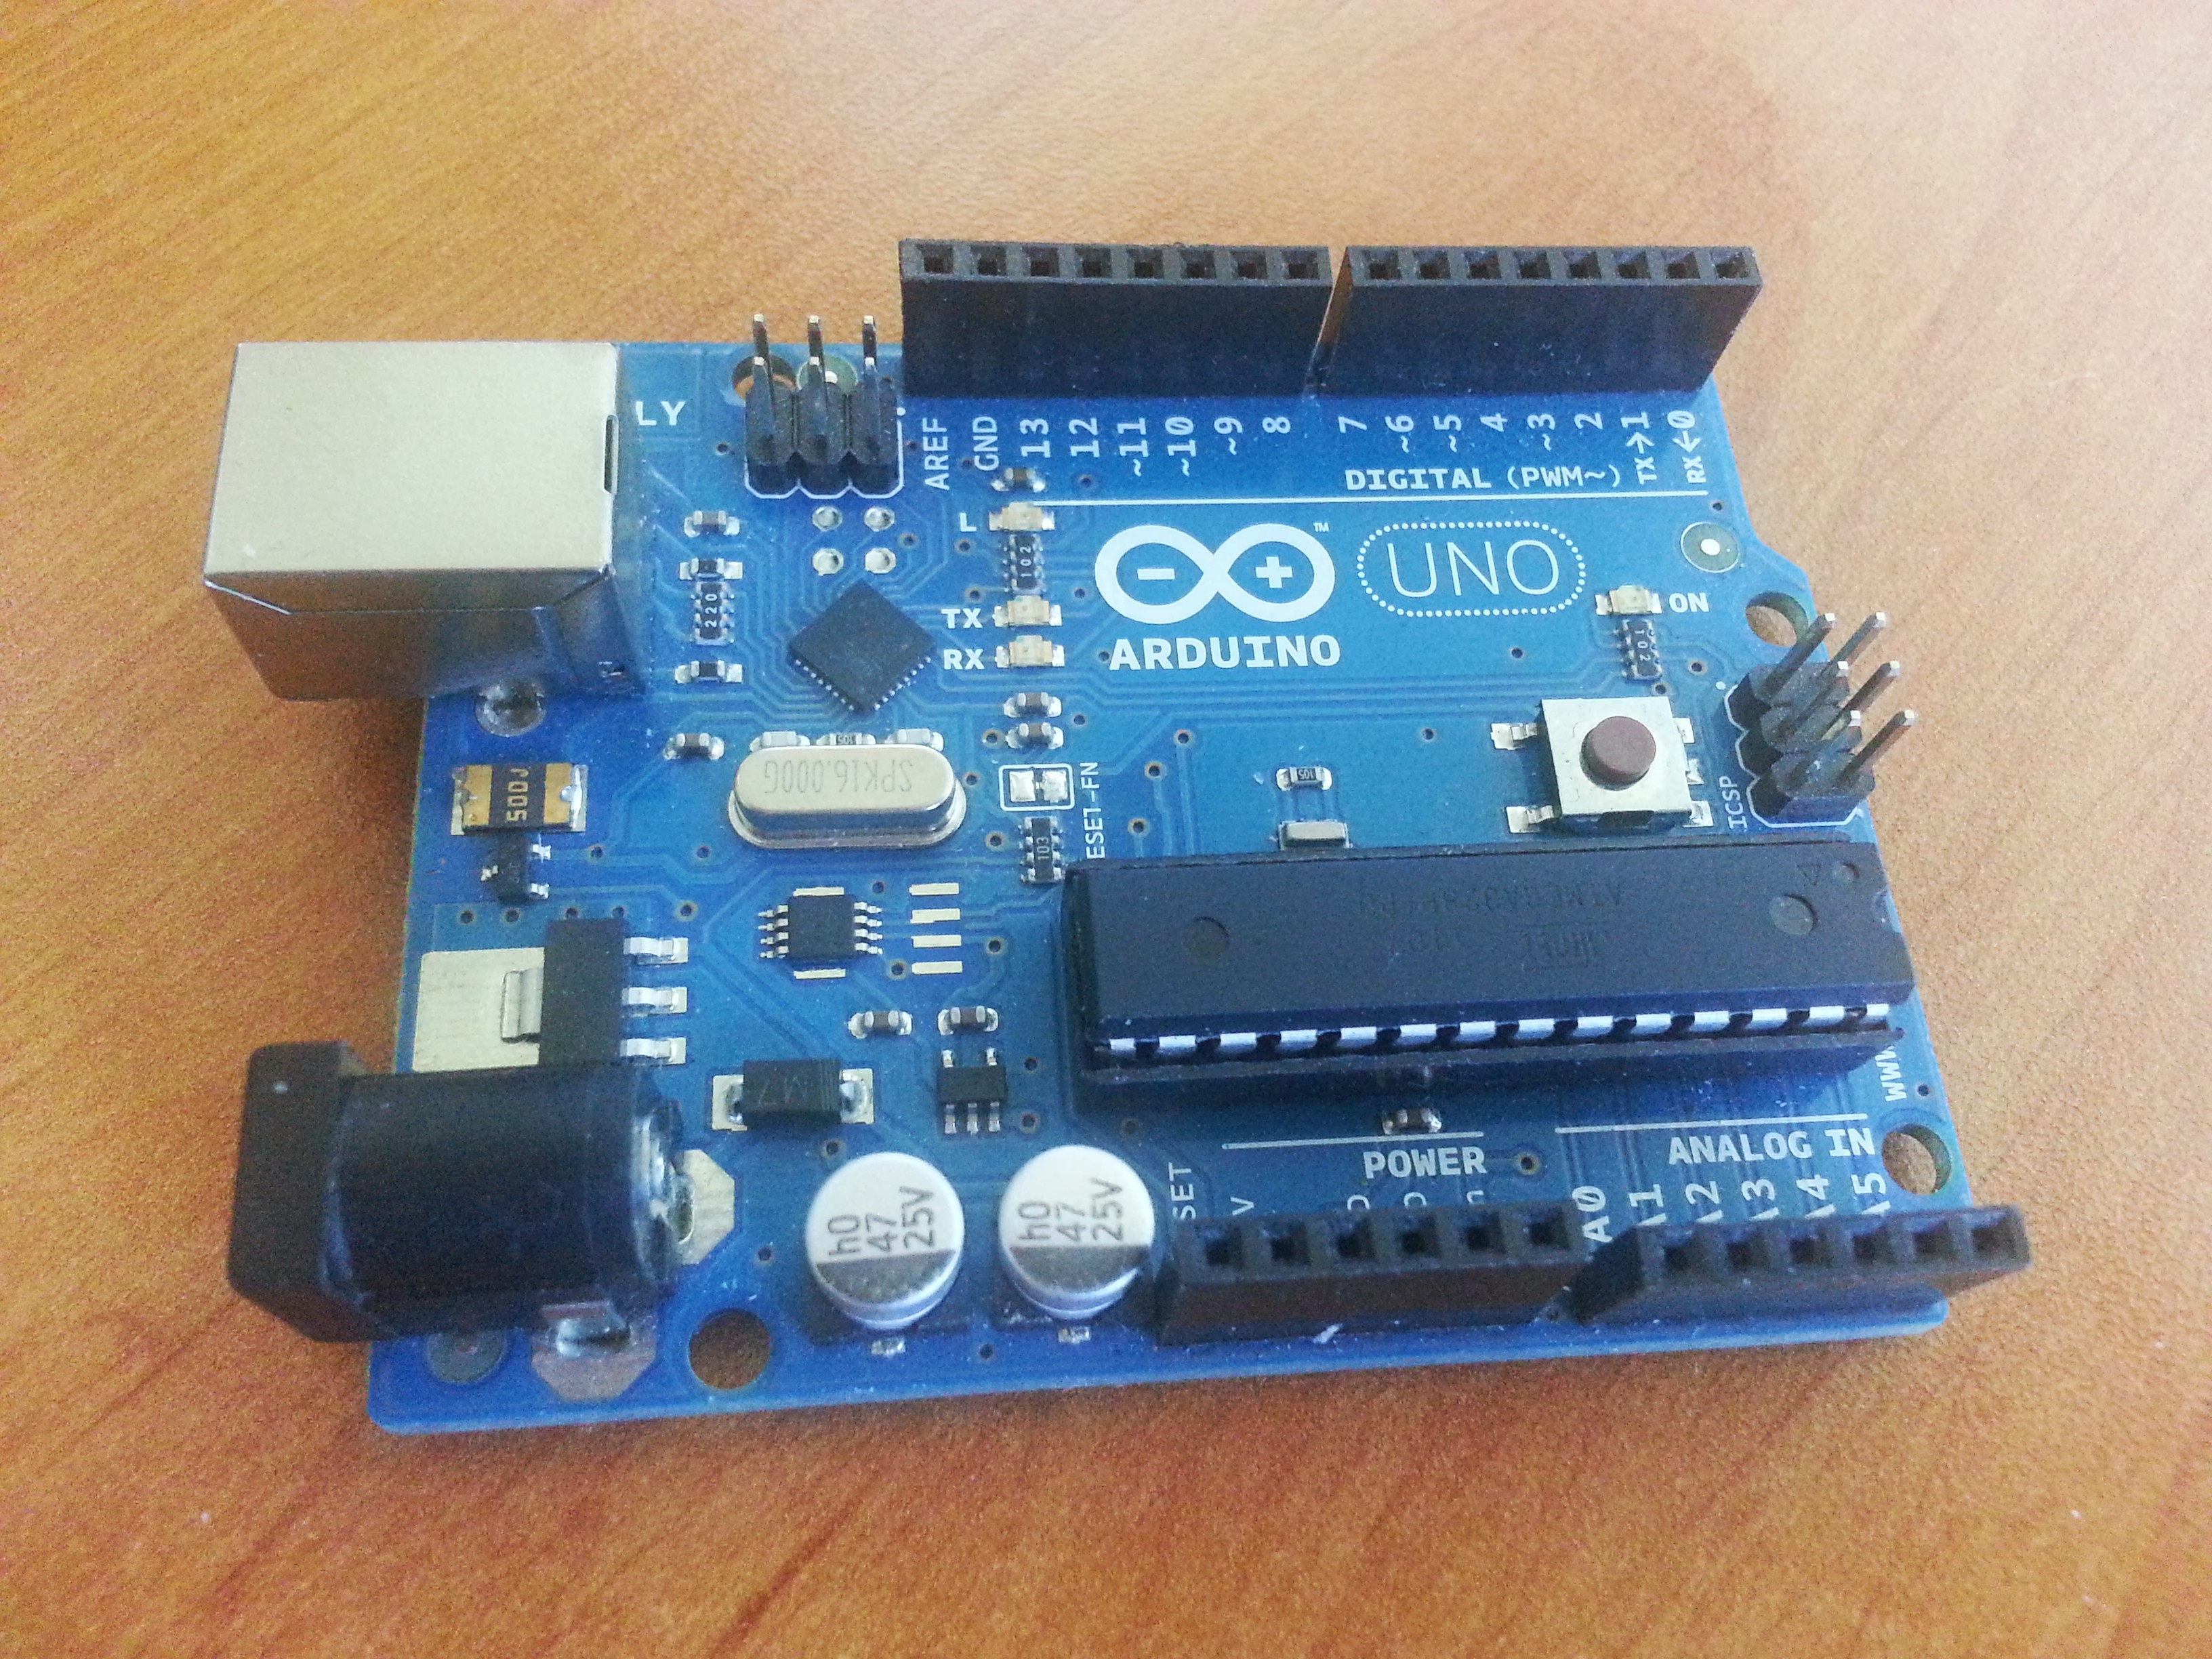
\includegraphics[width=3cm]{img/arduino.jpg}
        \item Raspberry Pi
            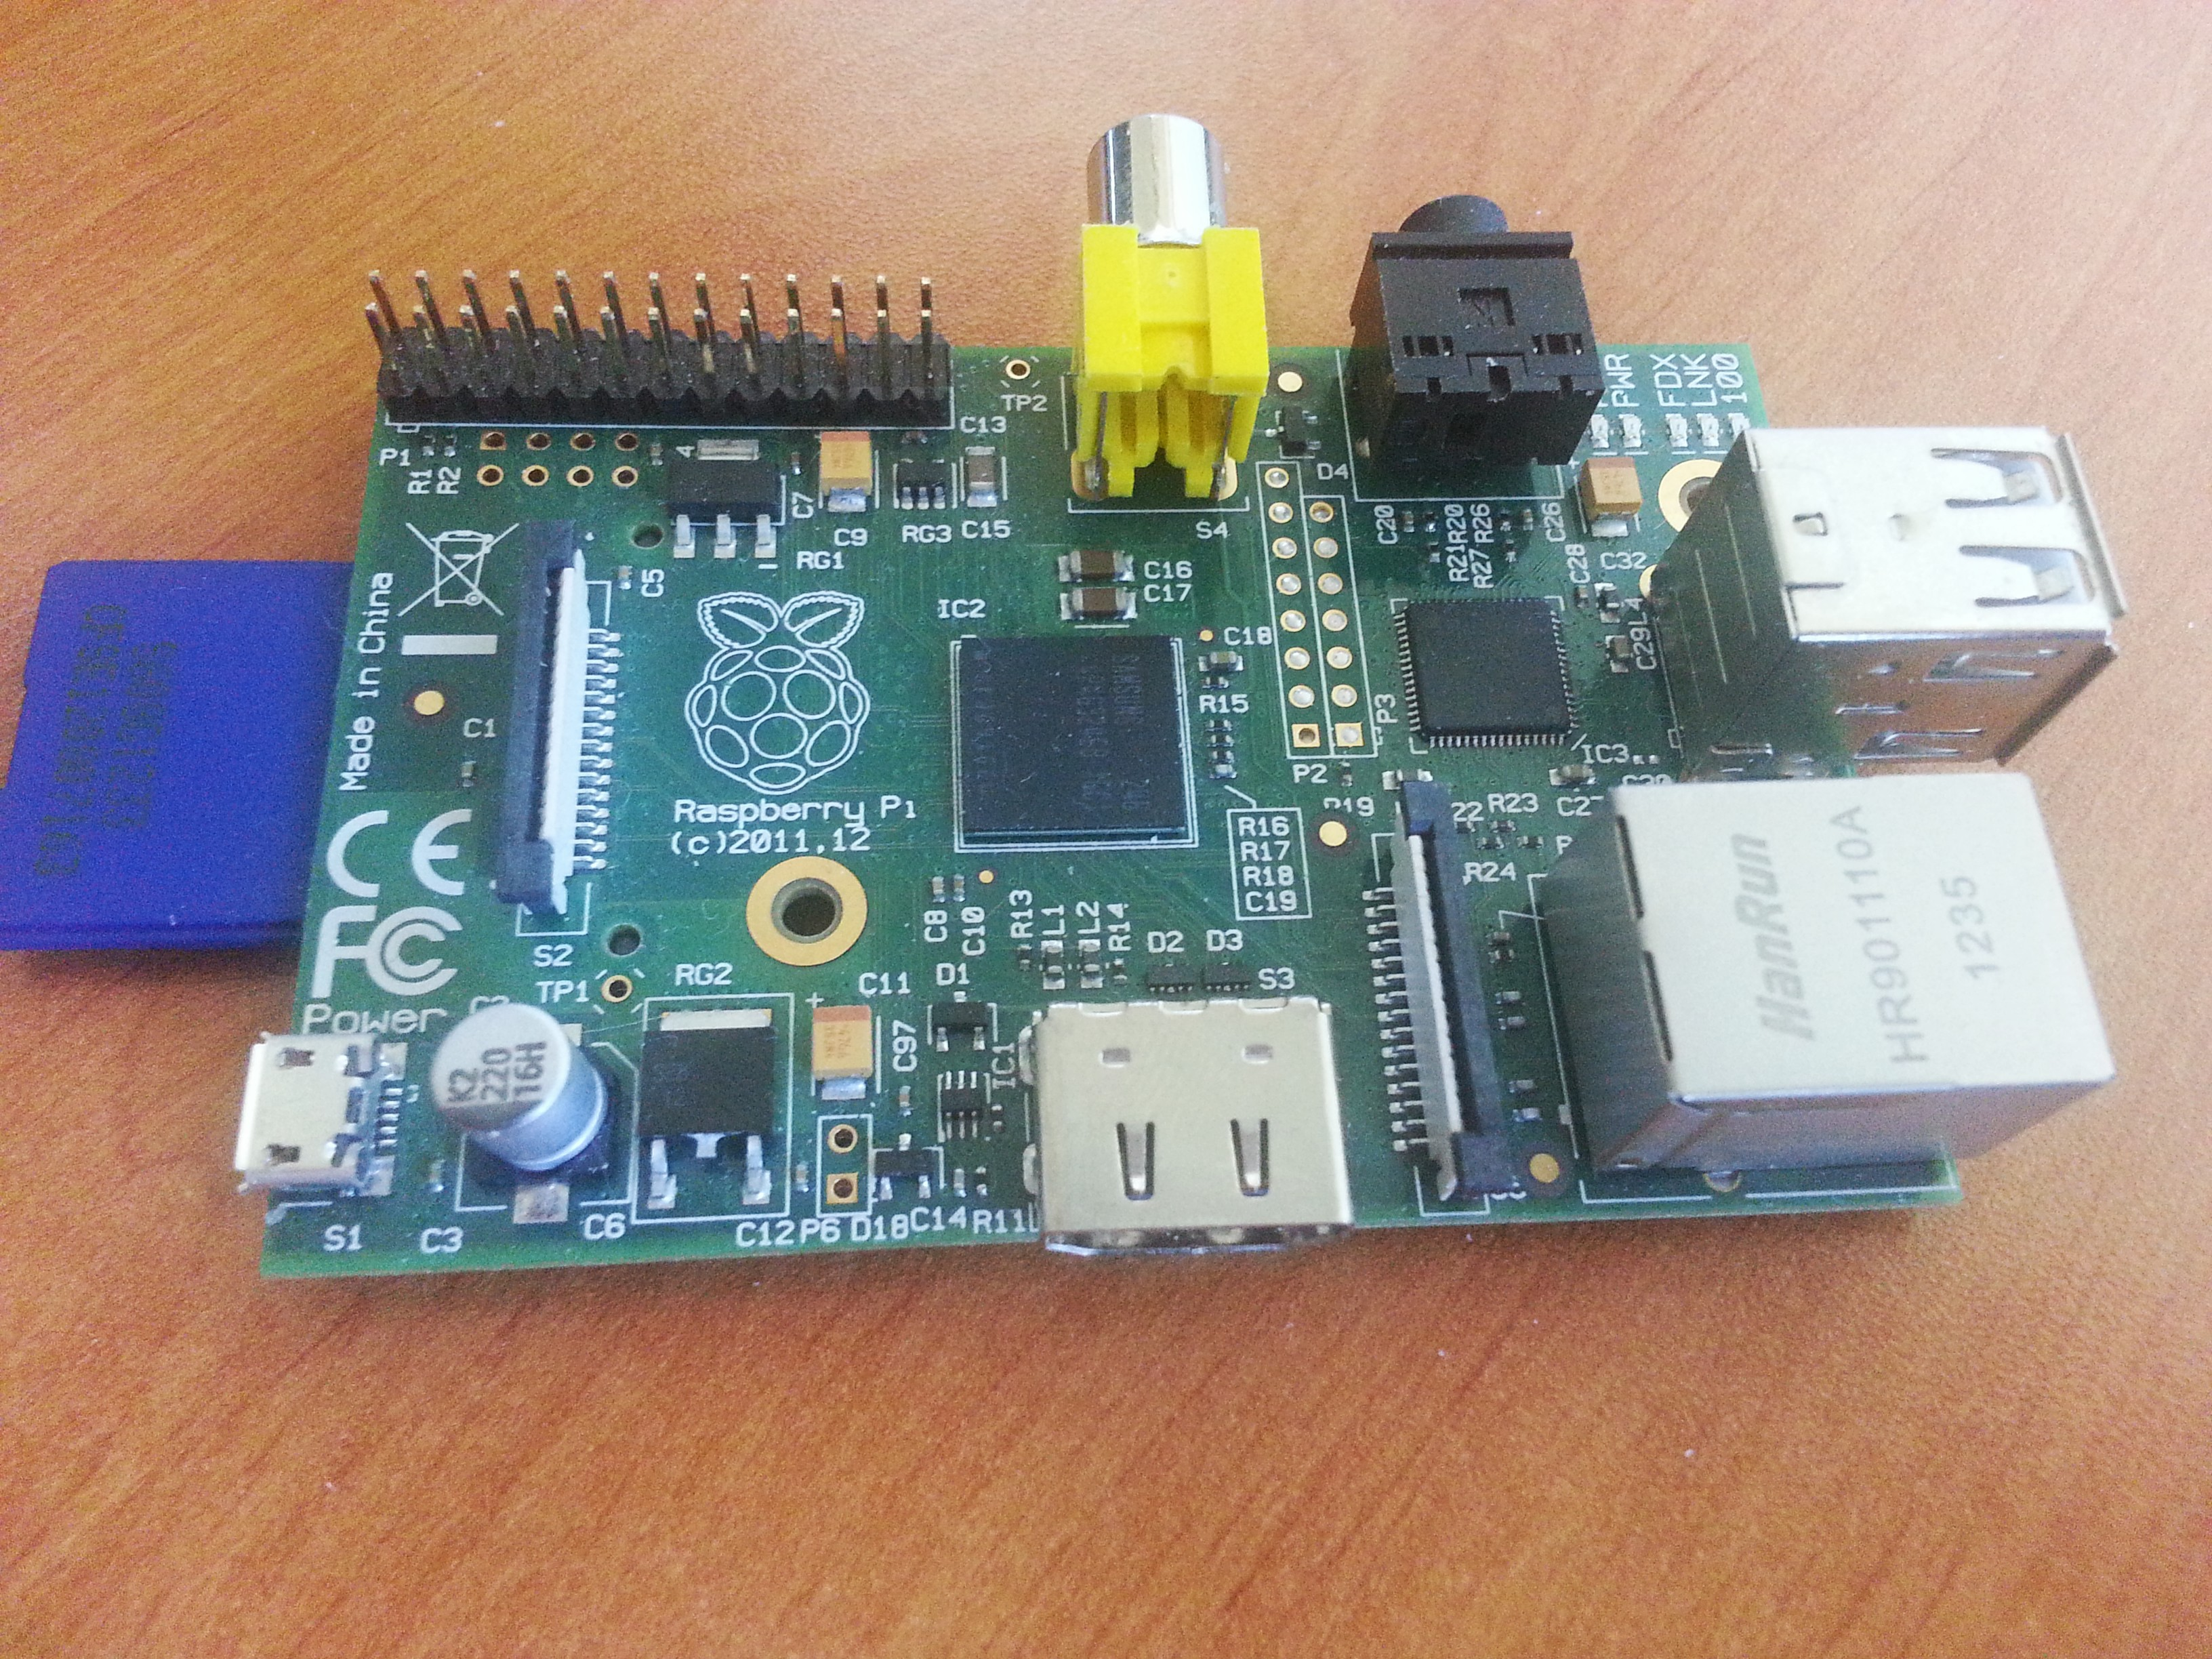
\includegraphics[width=3cm]{img/rpi.jpg}
        \item Mihini (via la ligne de commande et/ou Eclipse IDE)
        \item AirVantage
        \item API REST
    \end{itemize}
\end{frame}

\subsection{Conclusion}
\begin{frame}
    \frametitle{Résultats \& Intégration}
    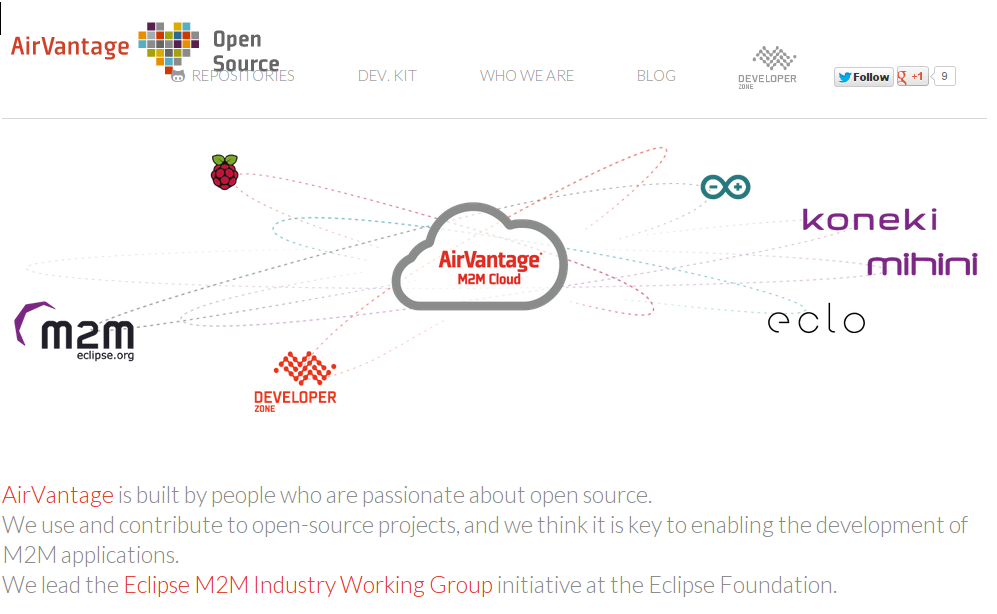
\includegraphics[width=\linewidth]{img/avgio.png}
\end{frame}

\section{Librairie MQTT pour MBED}

\begin{frame}
    \frametitle{Sommaire}
    \tableofcontents[currentsection, hideothersubsections]
\end{frame}

\subsection{Présentation}
\begin{frame}
    \frametitle{Présentation}
    \begin{block}{carte de base…}
        \begin{center}
            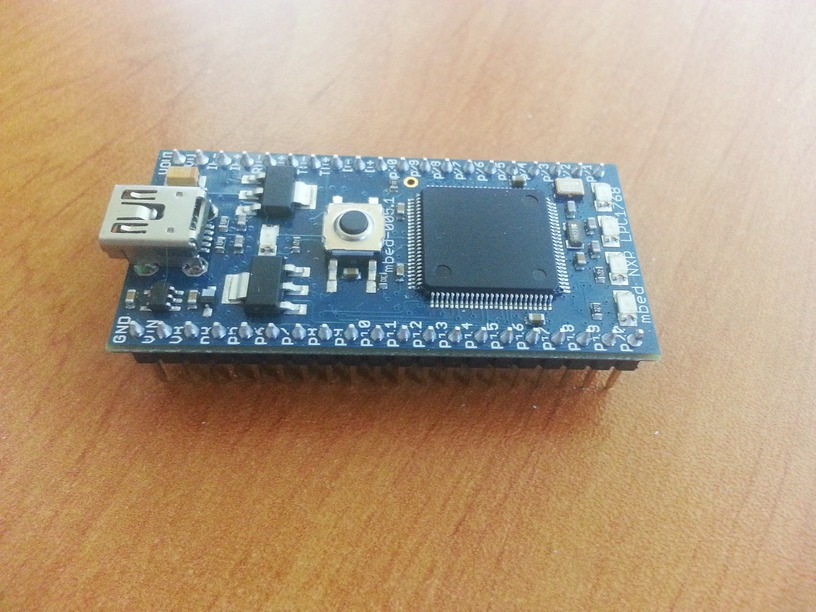
\includegraphics[width=3cm]{img/mbed.jpg}
        \end{center}
    \end{block}
    \begin{block}{… et son extension}
        \begin{center}
            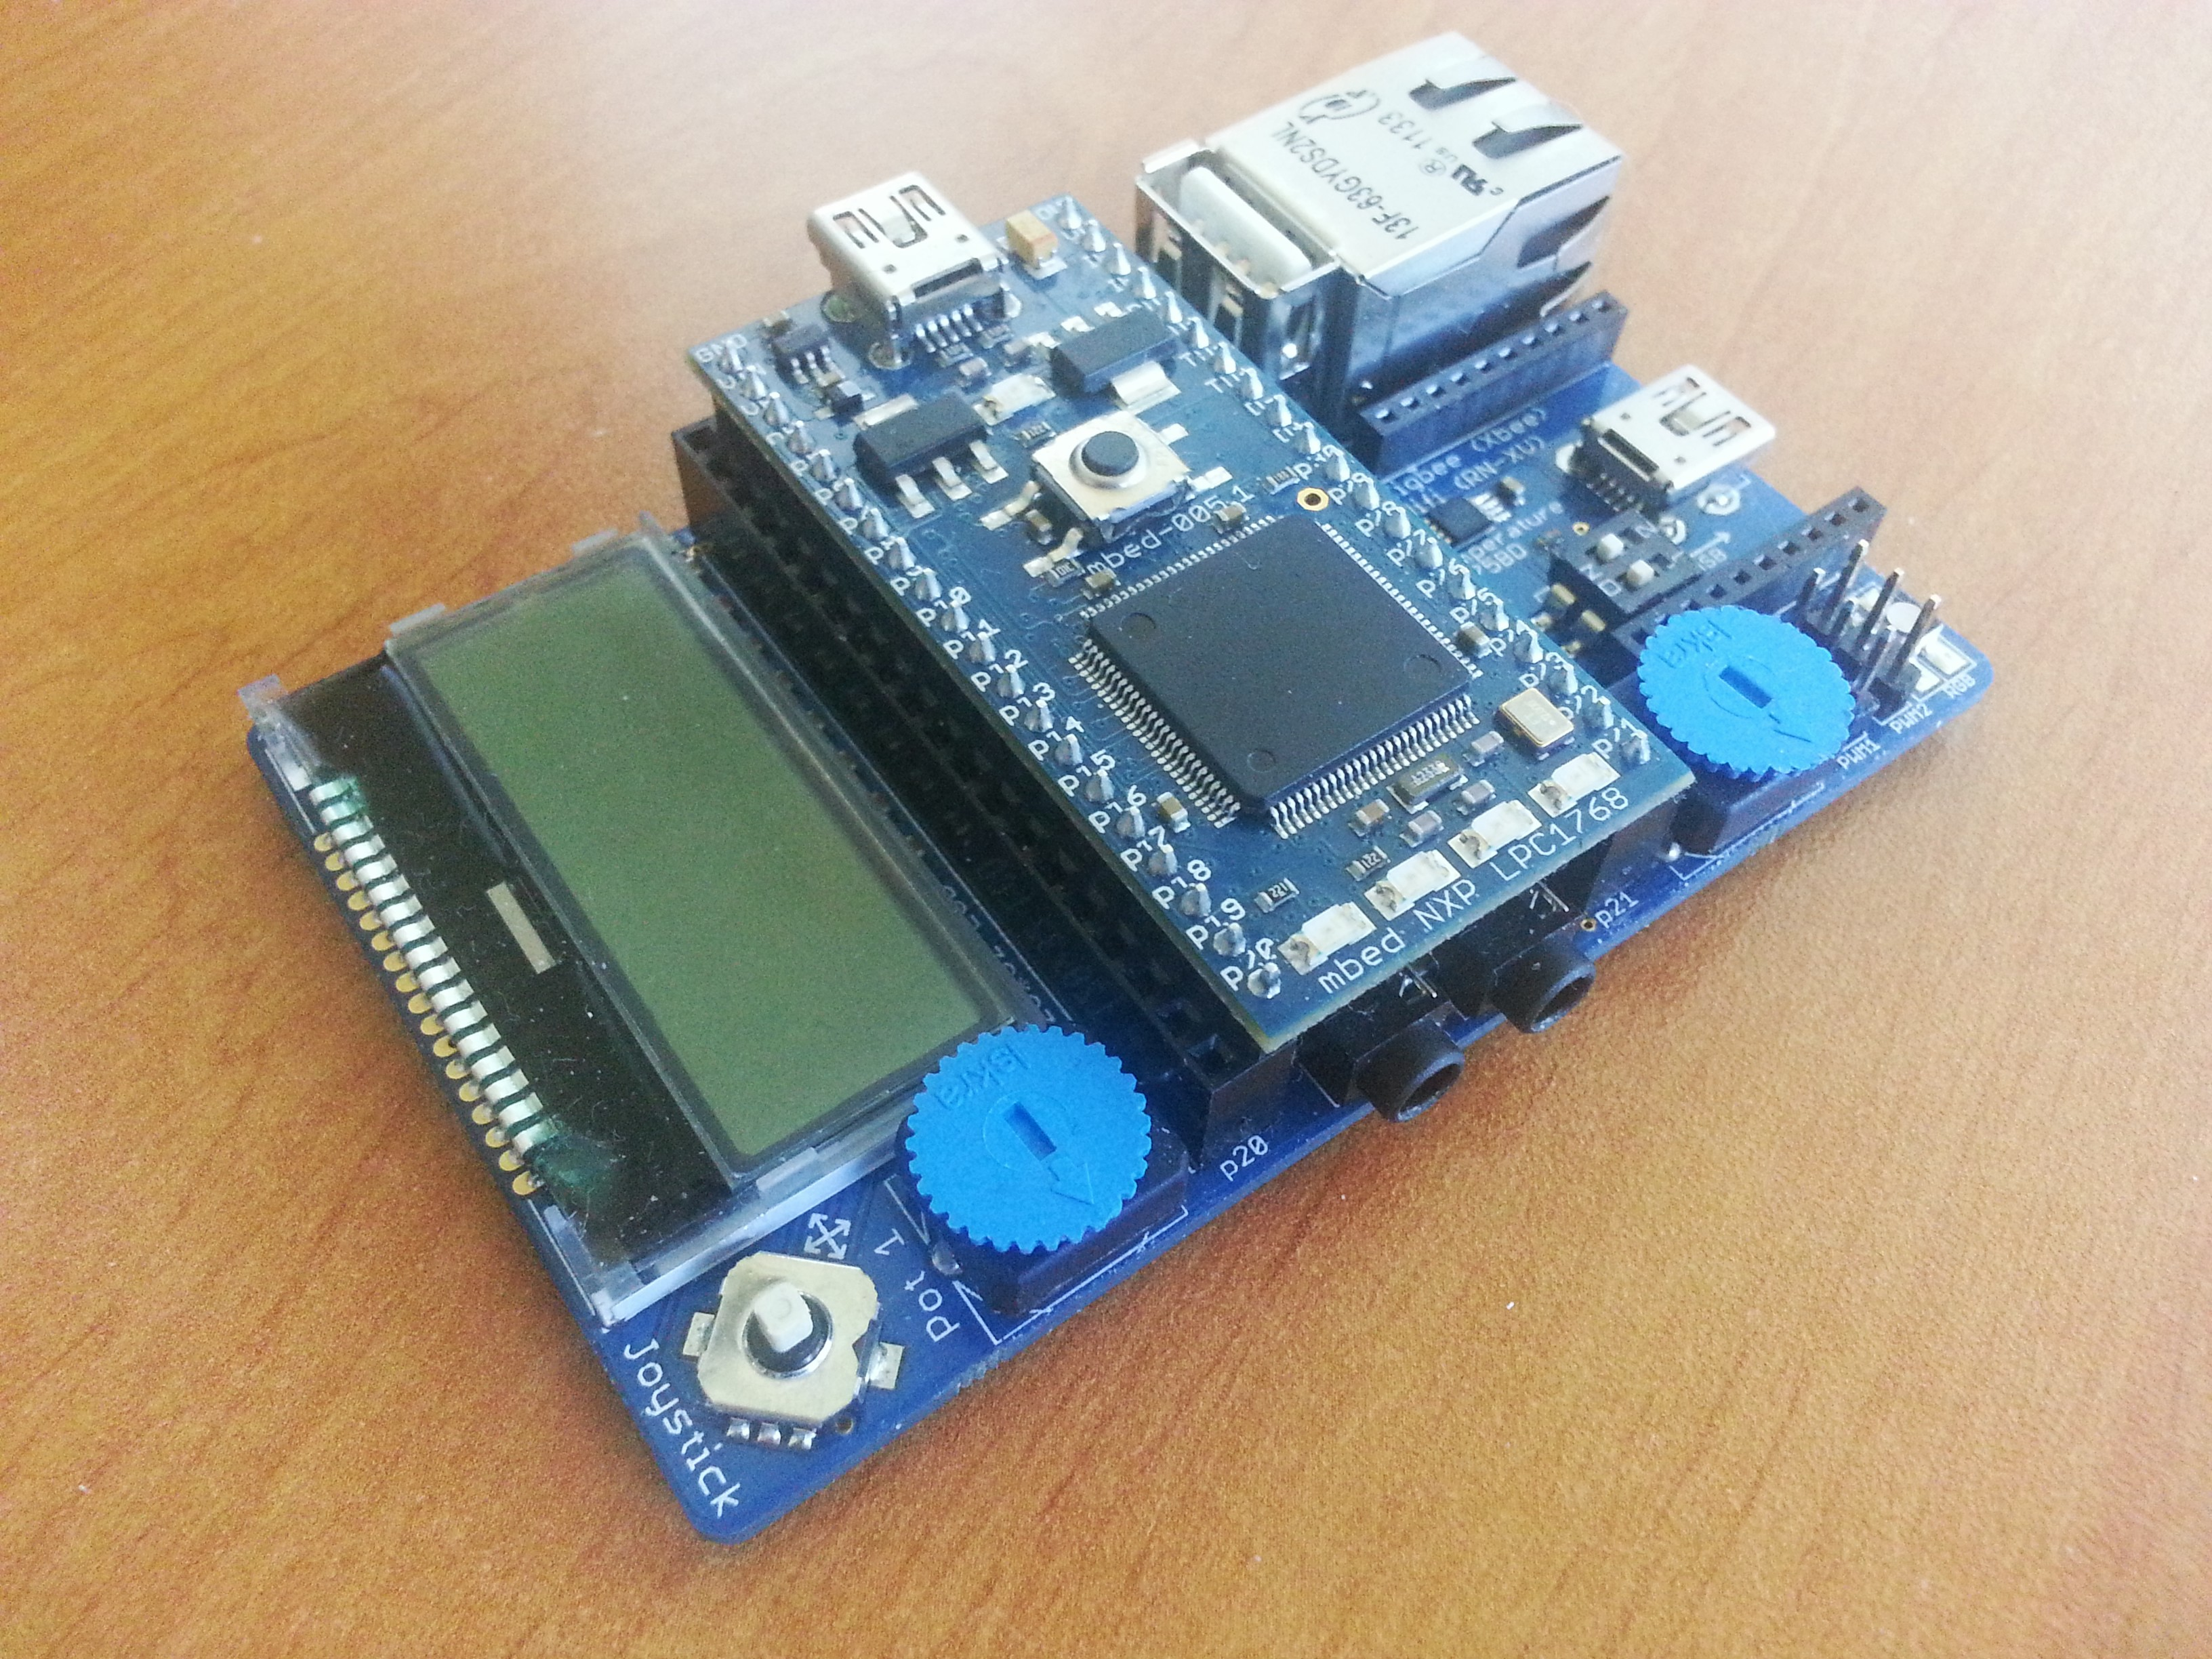
\includegraphics[width=3cm]{img/mbed_ext.jpg}
        \end{center}
    \end{block}
\end{frame}

\subsection{Conception}
\begin{frame}
    \frametitle{Principe}
    \begin{block}{Message Queue}
        \begin{center}
            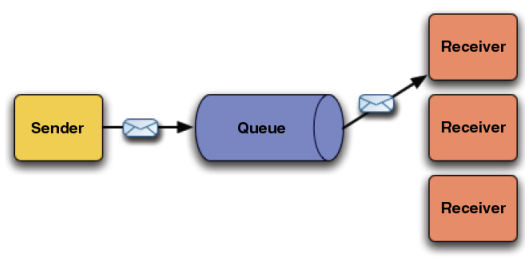
\includegraphics[height=3cm]{img/mq.png}
        \end{center}
    \end{block}
    \begin{block}{MQ Telemetry Transport}
        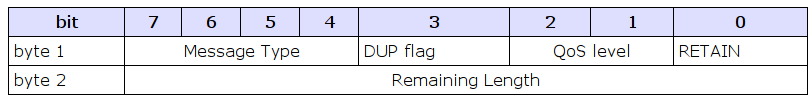
\includegraphics[width=\linewidth]{img/MQTT_header.png}
    \end{block}
\end{frame}

\subsection{Implémentation}
\begin{frame}
    \frametitle{Créations}
    \begin{block}{Librairies \& programmes d’exemple/test}
        \begin{itemize}
            \item niMQTT
            \item niMQTT\_example
            \item AV\_MQTT
            \item AV\_MQTT\_example
        \end{itemize}
    \end{block}
    \begin{block}{Disponibilité \& documentation}
        \begin{itemize}
            \item deux «notebooks»
            \item http://mbed.org/users/Nim65s/
        \end{itemize}
    \end{block}
\end{frame}

\section{Conclusion}

\begin{frame}
    \frametitle{Conclusion}
    % Questions
\end{frame}


\end{document}
